
\documentclass[letterpaper,twocolumn,10pt]{article}
\usepackage{usenix-2020-09}

% to be able to draw some self-contained figs
\usepackage{tikz}
\usepackage{amsmath}

% inlined bib file
\usepackage{filecontents}

% need to make the rectangle figures fit
\renewcommand{\dbltopfraction}{0.9}
\renewcommand{\dblfloatpagefraction}{0.8}
\setcounter{dbltopnumber}{3}


%-------------------------------------------------------------------------------
\begin{document}
%-------------------------------------------------------------------------------

%don't want date printed
\date{}

% make title bold and 14 pt font (Latex default is non-bold, 16 pt)
\title{\Large \bf Daily Mean and Variability of Hourly Temperature\\
  in Akron, Ohio, 2004--2026}

%for single author (just remove % characters)
\author{
{\rm Aaron Williams-Breth}\\
CYBR 515\\
awilliamsbreth@ewu.edu
} % end author

\maketitle

%-------------------------------------------------------------------------------
\begin{abstract}
%-------------------------------------------------------------------------------
This paper showcases 22 years of hourly temperature data for
Akron, Ohio, to see how temperature changes over a year and within a
single day. I calculated the mean and standard deviation of every day,
and plotted them alongside the raw readings at three different time scales: the
full record, one year, and one month.
\end{abstract}


%-------------------------------------------------------------------------------
\section{Introduction}
%-------------------------------------------------------------------------------
For this assignment I decided to look at temperature, as it is the weather variable where patterns are the easiest to see and to explain. Air temperature follows two cycles at once. Over a year it rises into summer and falls into winter, and over a single day it warms up after sunrise and cools back down overnight. I wanted to see both of theseccycles in real data, so I chose Akron, Ohio, which is where I am from,cand started the data in July 2004, the year I was born.

For every day in the data, I calculated the mean temperature and the standard deviation of that day's hourly readings. The daily mean follows the pattern of the seasons, while the daily standard deviation shows how much the temperature shifts during the day.

%-------------------------------------------------------------------------------
\section{Footnotes, Verbatim, and Citations}
%-------------------------------------------------------------------------------
\subsection{Data}

I pulled the data from the Open-Meteo Historical Weather API~\cite{openmeteo}. The API takes in a request with the location, the dates, and the weather variables wanted, then sends back the data. I requested the hourly variable \texttt{temperature\_2m}, which is the air temperature 2 meters above the ground, for latitude $41.08$ and longitude $-81.59$ (Akron, Ohio). The request covered July 27, 2004 to November 1, 2026, which is 22 years 2 months and 4 days of data. I set the temperatures to be in Fahrenheit, and the times to use Akron's local time zone (\texttt{America/New\_York}), so each day starts at local midnight.

\subsection{Calculations}

To describe each day, I calculated two numbers from that day's hourly readings. Let $x_1, x_2, \dots, x_n$ be the hourly temperatures for one day, where $n$ is the number of readings (24). The first number is the daily mean $\bar{x}$, which is the average of the readings,
\begin{equation}
  \bar{x} = \frac{1}{n} \sum_{i=1}^{n} x_i ,
  \label{eq:mean}
\end{equation}
and the second is the daily standard deviation $s$, which measures how far the readings spread out from that mean,
\begin{equation}
  s = \sqrt{\frac{1}{n-1} \sum_{i=1}^{n} \left(x_i - \bar{x}\right)^2 } .
  \label{eq:std}
\end{equation}

Equation~\ref{eq:std} is the sample standard deviation, which divides by $n-1$ instead of $n$. A large $s$ means the temperature swung a lot that day, while a small $s$ means the day stayed fairly steady.

The \texttt{pandas} \texttt{resample()} function groups the hourly readings into days, and then \texttt{mean()} and \texttt{std()} apply Equations~\ref{eq:mean} and~\ref{eq:std} to every day at once. Both numbers are calculated from all of the hourly readings, but for the plots I only kept one reading every 3 hours (00:00, 03:00, \dots, 21:00) as the raw data points. In the plots, each day's standard deviation is drawn as a shaded band from $\bar{x} - s$ to $\bar{x} + s$.

%-------------------------------------------------------------------------------
\section{Floating Figures and Lists}

\begin{figure*}[t]
  \centering
  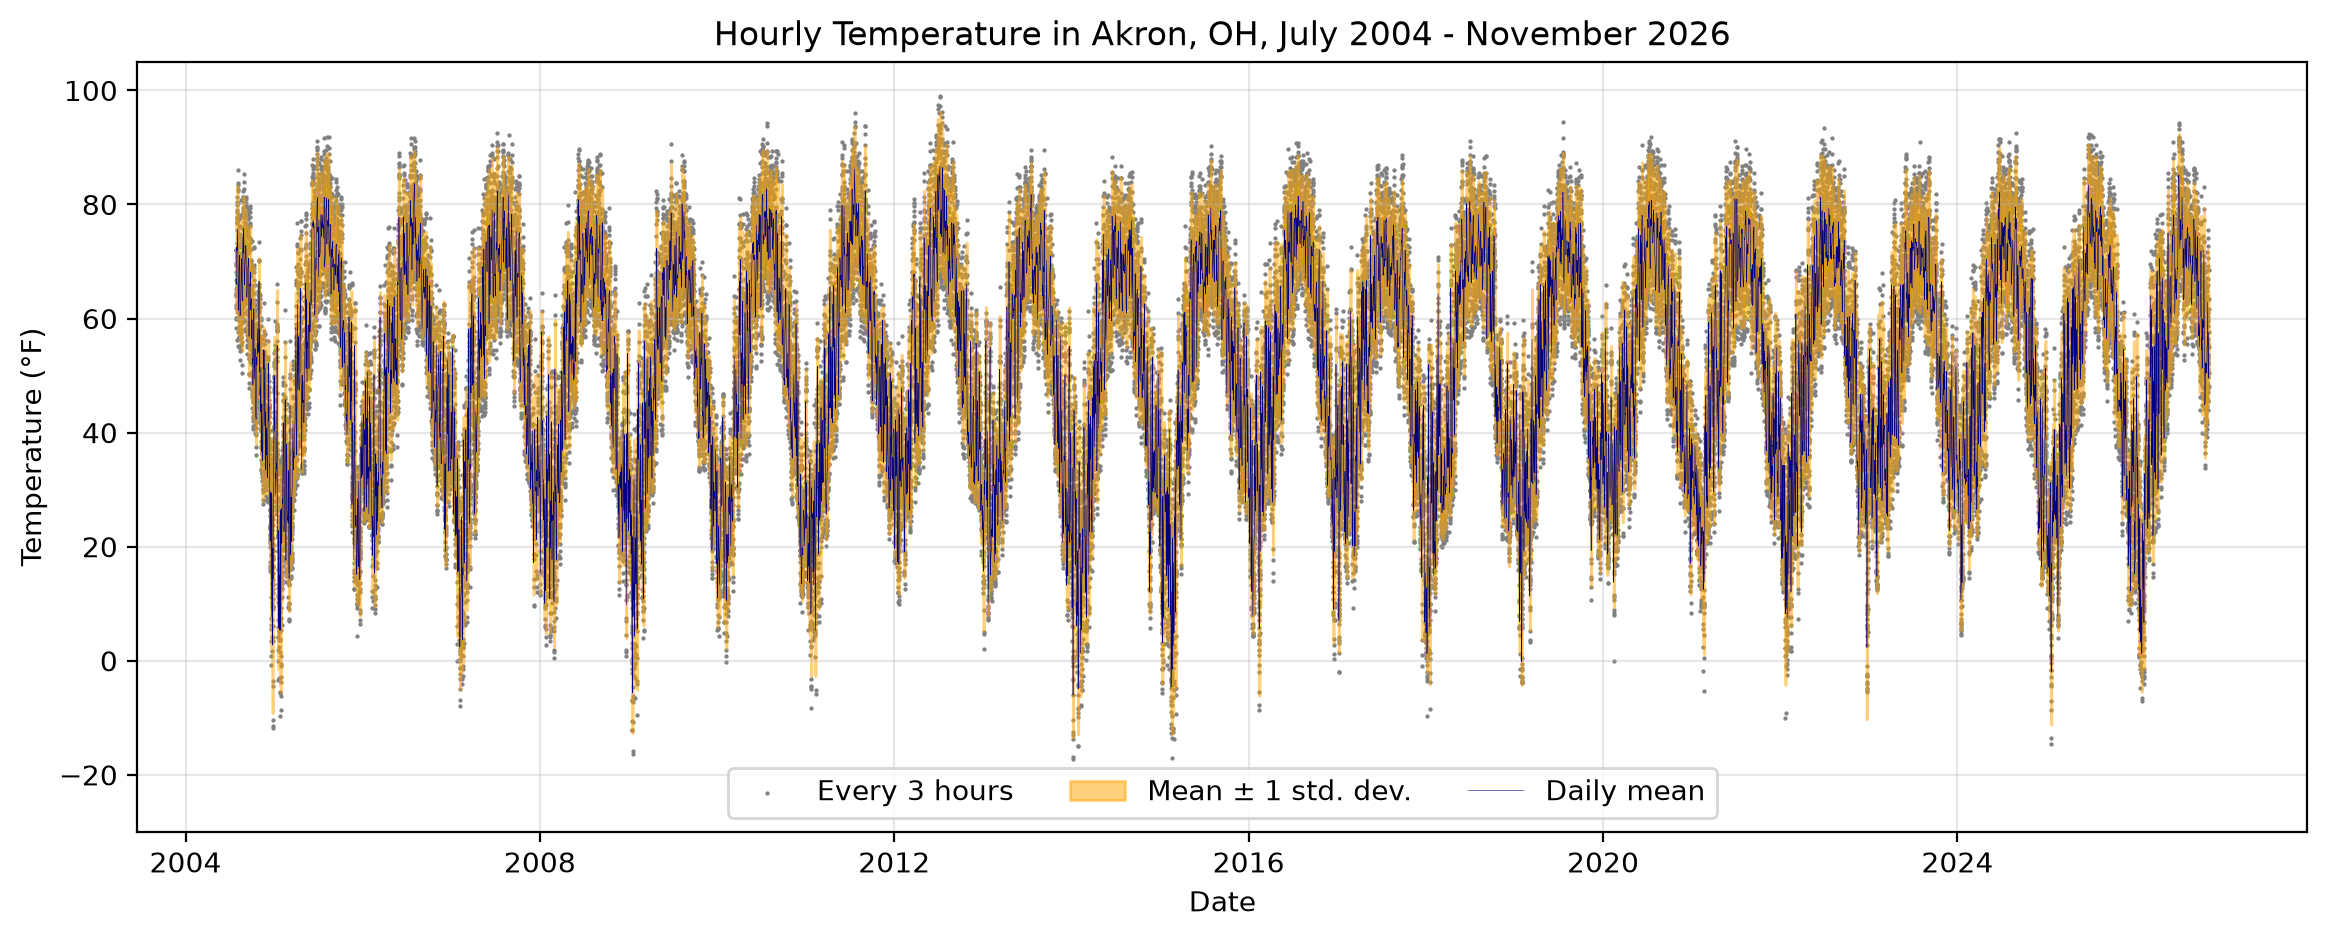
\includegraphics[width=\textwidth,height=0.23\textheight,keepaspectratio]{temperature_full.png}
  \caption{\label{fig:full} Hourly temperature in Akron, OH, July
    2004--November 2026. 
    Gray dots: readings every 3 hours. 
    Blue line:
    daily mean. 
    Orange band: daily mean $\pm$ 1 standard deviation.}
\end{figure*}

\begin{figure*}[t]
  \centering
  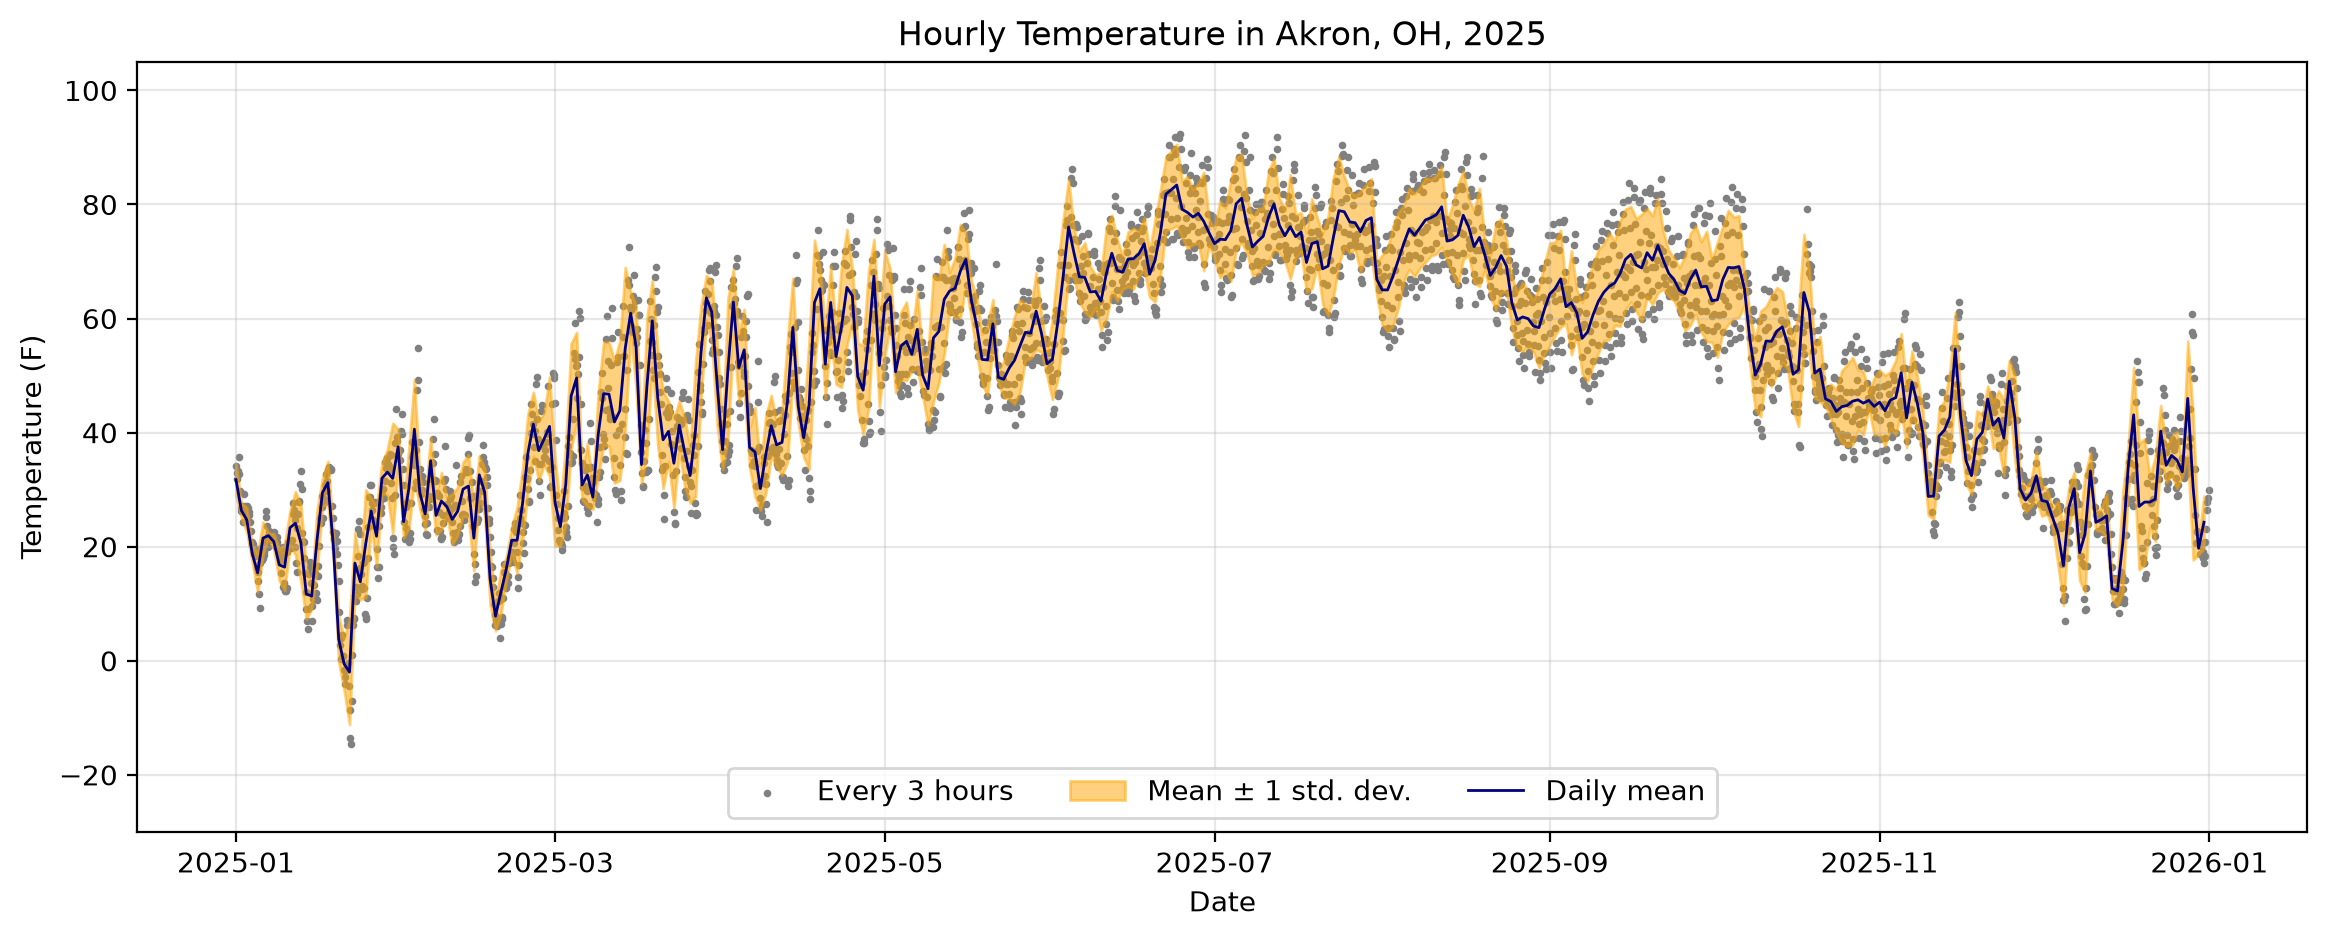
\includegraphics[width=\textwidth,height=0.23\textheight,keepaspectratio]{temperature_2025.png}
  \caption{\label{fig:year} Hourly temperature in Akron, OH, during 2025. 
    Gray dots: readings every 3 hours. 
    Blue line: daily mean. 
    Orange band: daily mean $\pm$ 1 standard deviation.}
\end{figure*}

\begin{figure*}[t]
  \centering
  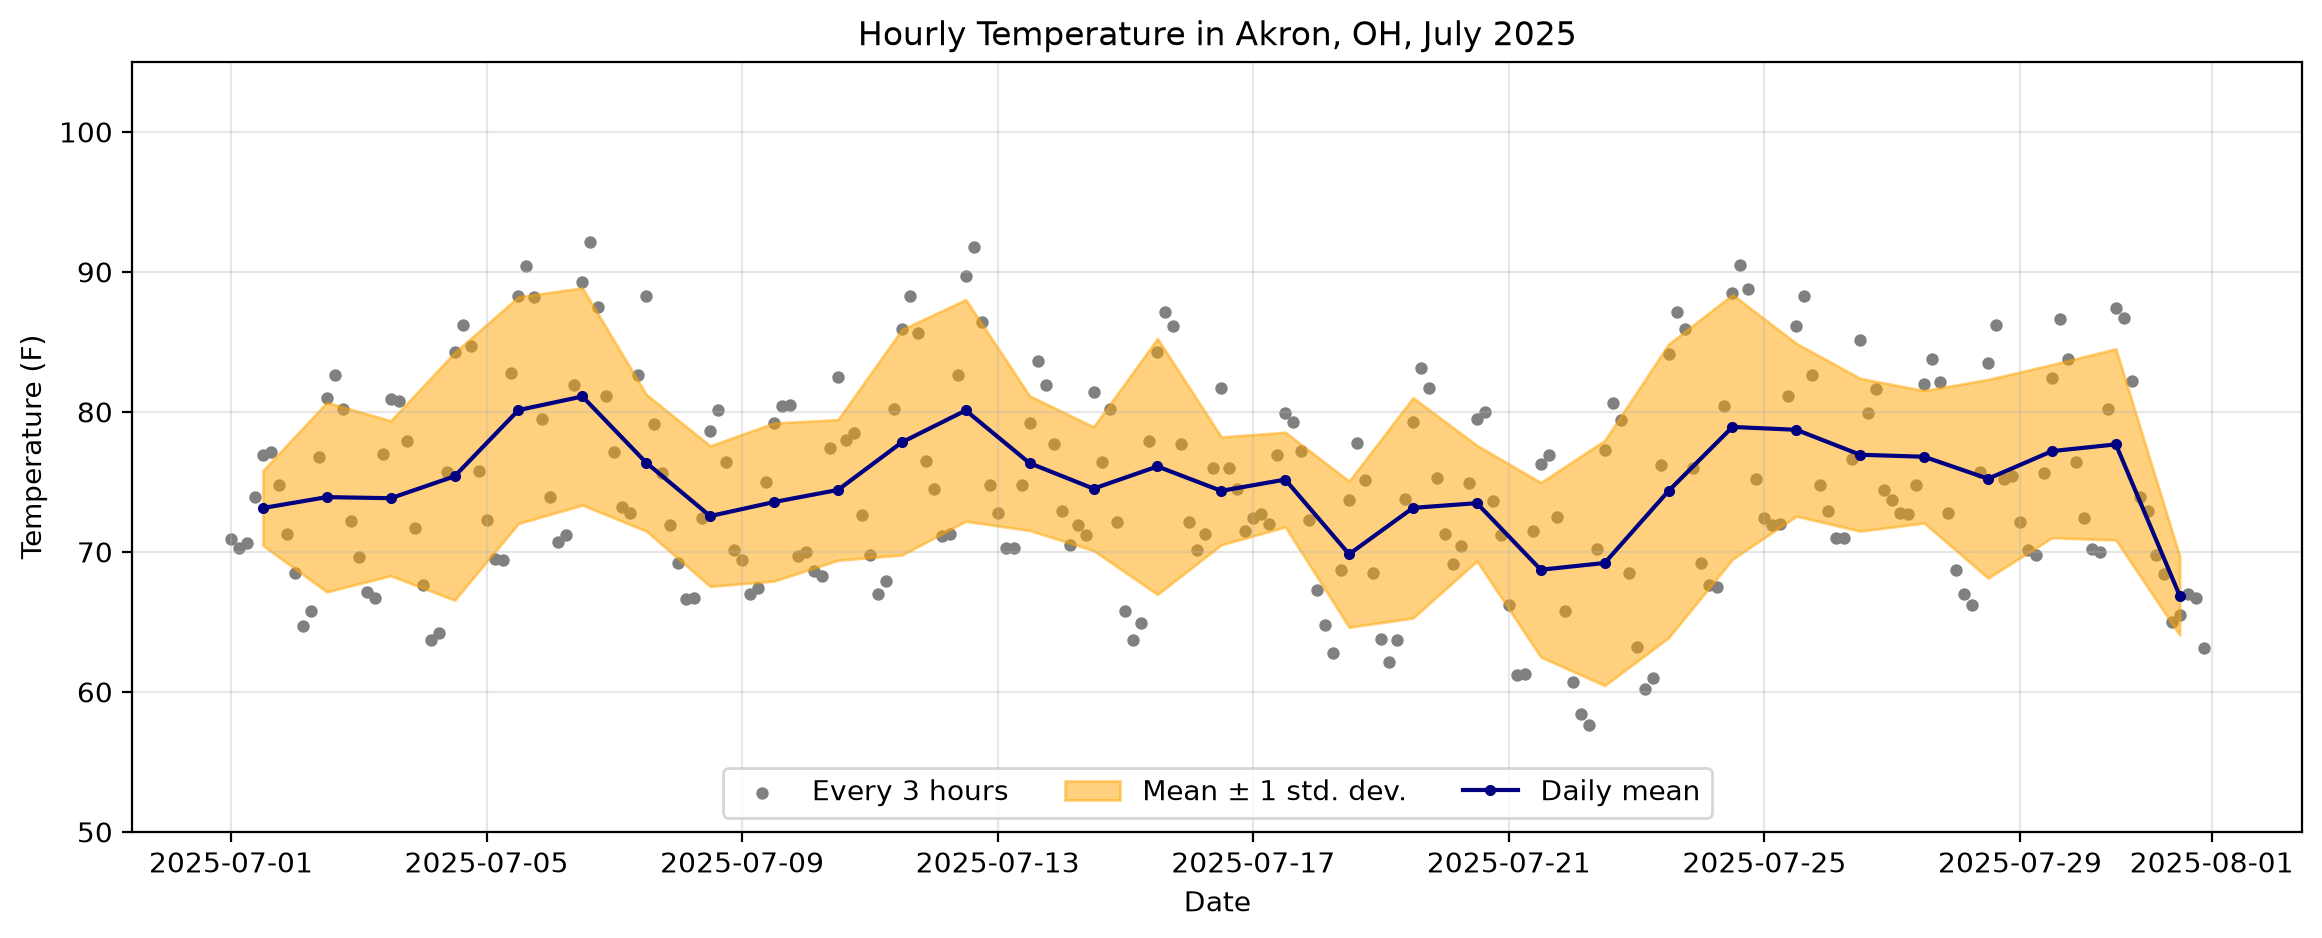
\includegraphics[width=\textwidth,height=0.23\textheight,keepaspectratio]{temperature_month.png}
  \caption{\label{fig:month} Hourly temperature in Akron, OH, during July
    2025.
    Gray dots: readings every 3 hours. 
    Blue line: daily mean. 
    Orange band: daily mean $\pm$ 1 standard deviation.}
\end{figure*}

I plotted the temperature data at three different scales, the full 22 year record, the entire 2025 year, and one month. In every figure, the gray dots are the raw readings every 3 hours, the blue line  is the daily mean (Equation~\ref{eq:mean}), and the orange band is the daily mean plus or minus  one standard deviation (Equation~\ref{eq:std}).

Figure~\ref{fig:full} shows the full 22 year record. The seasonly cycle is shown through the temperature rising to its peak each summer and drops to its lowest point each winter. Since 22 years are squeezed into  one plot, the details are hard to see, so the next figures zoom in.

Figure~\ref{fig:year} shows the entire year of 2025. At this scale, the spread of the gray dots around the daily mean is visible, and so is the day-to-day noise caused by passing weather systems.

Figure~\ref{fig:month} zooms in to July 2025. Each day now has its own step in the navy line and its own  section of the orange band. A tall band means a large standard deviation, so the temperature changed a lot that day. A short band means the temperature stayed steady.
%-------------------------------------------------------------------------------
\bibliographystyle{plain}
\bibliography{refs}

%%%%%%%%%%%%%%%%%%%%%%%%%%%%%%%%%%%%%%%%%%%%%%%%%%%%%%%%%%%%%%%%%%%%%%%%%%%%%%%%
\end{document}
%%%%%%%%%%%%%%%%%%%%%%%%%%%%%%%%%%%%%%%%%%%%%%%%%%%%%%%%%%%%%%%%%%%%%%%%%%%%%%%%

%%  LocalWords:  endnotes includegraphics fread ptr nobj noindent
%%  LocalWords:  pdflatex acks
